\documentclass[aspectratio=169, 9pt]{beamer}\usepackage[]{graphicx}\usepackage[]{color}
% maxwidth is the original width if it is less than linewidth
% otherwise use linewidth (to make sure the graphics do not exceed the margin)
\makeatletter
\def\maxwidth{ %
  \ifdim\Gin@nat@width>\linewidth
    \linewidth
  \else
    \Gin@nat@width
  \fi
}
\makeatother

\definecolor{fgcolor}{rgb}{0.345, 0.345, 0.345}
\newcommand{\hlnum}[1]{\textcolor[rgb]{0.686,0.059,0.569}{#1}}%
\newcommand{\hlstr}[1]{\textcolor[rgb]{0.192,0.494,0.8}{#1}}%
\newcommand{\hlcom}[1]{\textcolor[rgb]{0.678,0.584,0.686}{\textit{#1}}}%
\newcommand{\hlopt}[1]{\textcolor[rgb]{0,0,0}{#1}}%
\newcommand{\hlstd}[1]{\textcolor[rgb]{0.345,0.345,0.345}{#1}}%
\newcommand{\hlkwa}[1]{\textcolor[rgb]{0.161,0.373,0.58}{\textbf{#1}}}%
\newcommand{\hlkwb}[1]{\textcolor[rgb]{0.69,0.353,0.396}{#1}}%
\newcommand{\hlkwc}[1]{\textcolor[rgb]{0.333,0.667,0.333}{#1}}%
\newcommand{\hlkwd}[1]{\textcolor[rgb]{0.737,0.353,0.396}{\textbf{#1}}}%
\let\hlipl\hlkwb

\usepackage{framed}
\makeatletter
\newenvironment{kframe}{%
 \def\at@end@of@kframe{}%
 \ifinner\ifhmode%
  \def\at@end@of@kframe{\end{minipage}}%
  \begin{minipage}{\columnwidth}%
 \fi\fi%
 \def\FrameCommand##1{\hskip\@totalleftmargin \hskip-\fboxsep
 \colorbox{shadecolor}{##1}\hskip-\fboxsep
     % There is no \\@totalrightmargin, so:
     \hskip-\linewidth \hskip-\@totalleftmargin \hskip\columnwidth}%
 \MakeFramed {\advance\hsize-\width
   \@totalleftmargin\z@ \linewidth\hsize
   \@setminipage}}%
 {\par\unskip\endMakeFramed%
 \at@end@of@kframe}
\makeatother

\definecolor{shadecolor}{rgb}{.97, .97, .97}
\definecolor{messagecolor}{rgb}{0, 0, 0}
\definecolor{warningcolor}{rgb}{1, 0, 1}
\definecolor{errorcolor}{rgb}{1, 0, 0}
\newenvironment{knitrout}{}{} % an empty environment to be redefined in TeX

\usepackage{alltt}

% \transdissolve[duration=0.2] % Only works with Adobe Acrobat

% \mode<handout>

% Some important packages
\usepackage{epstopdf}
\hypersetup{colorlinks=false, allcolors=purple}
\usepackage{booktabs}
\linespread{1.3}
\usepackage{tabularx}
\usepackage{makecell} % For makecell within tables
\usepackage{geometry}
\usepackage{algorithm2e}
\usepackage{amsmath, amssymb}
% Mathematical functions
% DELETED!
\renewcommand{\Pr}[1]{{\mathbb{P}\left(#1\right) }}
% DELETED!
% DELETED!
% DELETED!
% DELETED!
% DELETED!

% DELETED!
\newcommand{\sufstats}[1]{s\left(#1\right)}
\renewcommand{\exp}[1]{\mbox{exp}\left\{#1\right\}}
\newcommand{\transpose}[1]{{#1}^\mathbf{t}}

% Objects
% DELETED!
% DELETED!
\newcommand{\Graph}{\mathbf{G}}
\newcommand{\graph}{\mathbf{g}}
\newcommand{\GRAPH}{\mathcal{G}}
\newcommand{\Adjmat}{Y}
\newcommand{\adjmat}{y}
\newcommand{\ADJMAT}{\mathcal{Y}}

\newcommand{\INDEPVAR}{\mathcal{X}}
\newcommand{\Indepvar}{X}
\newcommand{\indepvar}{x}

\newcommand{\normconst}{\kappa\left(\params, \Indepvar\right)}

\graphicspath{{./figures/}{.}{./terms/}}


%% NEED THIS FOR CANCY TEX
\usepackage{pstricks}

% Colors
\definecolor{USCCardinal}{HTML}{990000} % 153 0 0 in RGB
\definecolor{USCGold}{HTML}{FFCC00}
\definecolor{USCGray}{HTML}{CCCCCC}

% To use the function \sout
\usepackage{ulem}
\usepackage{tabularx, booktabs}

% \bibliography{bibliography.bib}

\def\ergmito{ERGM\textit{ito}}
\def\ergmitos{\ergmito{}\textit{s}}
% Mathematical functions
\newcommand{\isone}[1]{{\boldsymbol{1}\left( #1 \right)}}
\renewcommand{\Pr}[1]{{\mathbb{P}\left(#1\right) }}
\newcommand{\f}[1]{{f\left(#1\right) }}
\newcommand{\Prcond}[2]{{\mathbb{P}\left(#1\vphantom{#2}\;\right|\left.\vphantom{#1}#2\right)}}
\newcommand{\fcond}[2]{{f\left(#1|#2\right) }}
\newcommand{\Expected}[1]{{\mathbb{E}\left\{#1\right\}}}
\newcommand{\ExpectedCond}[2]{{\mathbb{E}\left\{#1\vphantom{#2}\right|\left.\vphantom{#1}#2\right\}}}
\renewcommand{\exp}[1]{\mbox{exp}\left\{#1\right\}}

\newcommand{\Likelihood}[2]{\text{L}\left(#1 \left|\vphantom{#1}#2\right.\right)}

% Mathematical Annotation -------------------------------
% Modify this so that it matches the P01 convention overall

% Tree
\newcommand{\phylo}{\Lambda{}} % The actual tree
\newcommand{\aphylo}{D{}}      % The annotated phylogenetic tree
\newcommand{\aphyloObs}{\tilde \aphylo{}} % The observed annotated phylogenetic tree
\newcommand{\parent}[1]{\mathbf{p}\left(#1\right)}
\newcommand{\offspring}[1]{\mathbf{O}\left(#1\right)}
\newcommand{\nodes}{\mathcal{N}{}}
\newcommand{\edges}{\mathcal{E}{}}

\newcommand{\class}[1]{C_{#1}{}}

% Annotations
\newcommand{\Ann}{\mathbf{X}{}} % Matrix of "real" annotations
\newcommand{\ann}[1]{x_{#1}{}} % single element of "real" annotations
\newcommand{\constraints}{\mathcal{C}{}} % Taxon constraints

% Obs Annotations
\newcommand{\AnnObs}{\mathbf{Z}{}}%{Z{}} \mathbf{X}^{obs}{}
\newcommand{\annObs}[1]{z_{#1}{}}%{z{}}  x_{#1}^{obs

% Pred. Annotations
\newcommand{\AnnPred}{\hat X{}}
\newcommand{\annPred}[1]{\hat x_{#1}}

% Leaf nodes
\newcommand{\Leaf}{L{}}

% Shortest path
\newcommand{\Geodesic}{\text{T}{}}
\newcommand{\geodesic}{\tau{}}

\newcommand{\Params}{\Omega{}}
\newcommand{\params}{\omega{}}

% Parameters
\newcommand{\gain}{\mu_{01}{}}
\newcommand{\loss}{\mu_{10}{}}
\newcommand{\misszero}{\psi_{01}{}}
\newcommand{\missone}{\psi_{10}{}}
\newcommand{\proot}{\pi}


\usepackage[style=authoryear-comp]{biblatex}
\addbibresource{bibliography.bib}
% \renewcommand{\bibsection}{\subsubsection*{\bibname } }


% Styles
\usepackage{xcolor}
\usepackage{colortbl}
\definecolor{suffstat}{RGB}{10,159,0}
\definecolor{normconst}{RGB}{87,38,231}
\setbeamercolor{conclusions}{bg=usclightgray!60!white, fg=uscdarkgray}

% Noice!
\usetheme{usckeck}

\title[Stat. Comp. for Complex Systems]{Essays on Bioinformatics and
Social Network Analysis
\linebreak{\small Statistical and Computational Methods for
Complex Systems}}
\author[GGVY]{George G Vega Yon}
\institute[USC-PREVMED]{University of Southern California, Department of Preventive Medicine}
\date{November 18, 2019}

% Some definitions
\def\cursection{\frame{\frametitle{Contents}\tableofcontents[current]}}
\newcommand{\ergmpkg}[0]{\texttt{ergm}}
\newcommand{\ergmitopkg}[0]{\texttt{ergmito}}
\newcommand{\aphylopkg}[0]{\texttt{aphylo}}
\graphicspath{{.}{fig/}}


% ------------------------------------------------------------------------------
% ------------------------------------------------------------------------------
% --------------------------- END OF PREAMBLE ----------------------------------
% ------------------------------------------------------------------------------
% ------------------------------------------------------------------------------
\setbeamertemplate{note page}[plain]
%\setbeameroption{show notes}
\usepackage{pgfpages}
% \setbeameroption{show notes on second screen}

\newcommand{\hlc}[2]{{\only<#1>{\cellcolor{gray!50} #2}}}
\newcommand{\nhlc}[2]{{\only<#1>{#2}}}
\IfFileExists{upquote.sty}{\usepackage{upquote}}{}
\begin{document}
% \SweaveOpts{concordance=TRUE}

% ------------------------------------------------------------------------------
\begin{frame}%[noframenumbering]
\maketitle
\end{frame}

% ------------------------------------------------------------------------------
\begin{frame}
\frametitle{What motivates my research}

\begin{center}
\large
\textcolor{usccardinal}{\bf Statistical and computational methods for\\ %
bioinformatics and social network analysis}
\end{center}

\begin{itemize}[<+->]
\item We live in a non-{\it IID} world.
\item In some times, the cannot understand a process unless we look at it as a whole.
\item There's a reason why we usually assume {\it IID}.
\item {\it Modern} (as of today) computational tools help us coping with that.
\end{itemize}
\end{frame}


\frame{\frametitle{Contents}\tableofcontents}

% ------------------------------------------------------------------------------
\section{Paper 1: On the prediction of gene functions using phylogenetic trees}

\begin{frame}[t]
\usebeamertemplate{section intro}{}{}
\textcolor{uscgold}{
\Large {\bf On the prediction of gene functions using phylogenetic trees} \vskip0.25em
\large \textit{Joint with}: Paul D Thomas, Paul Marjoram, Huaiyu Mi, Duncan Thomas, and John Morrison
}
\end{frame}

% ------------------------------------------------------------------------------
\begin{frame}
\frametitle{Genes}

Encode the synthesis of genetic products that ultimately are related to a
particular aspect of life, for example

\def\tmpwidth{.9\linewidth}

\begin{table}
\begin{tabular}{*{3}{m{.31\linewidth}<{\centering}}}
\onslide<2->\bf Molecular function & %
\onslide<3->\bf Cellular component & %
\onslide<4->\bf Biological process \\
\onslide<2->\href{http://amigo.geneontology.org/amigo/term/GO:0005215}{Active transport GO:0005215}& %
\onslide<3->\href{http://amigo.geneontology.org/amigo/term/GO:0004016}{Mitochondria GO:0004016} & %
\onslide<4->\href{http://amigo.geneontology.org/amigo/term/GO:0060047}{Heart contraction GO:0060047} \\
\onslide<2->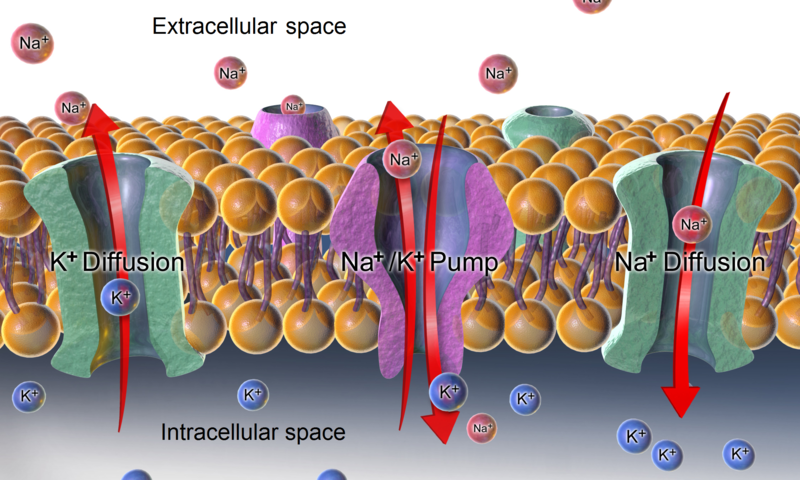
\includegraphics[width=\tmpwidth]{Sodium-potassium_pump_and_diffusion.png} & %
\onslide<3->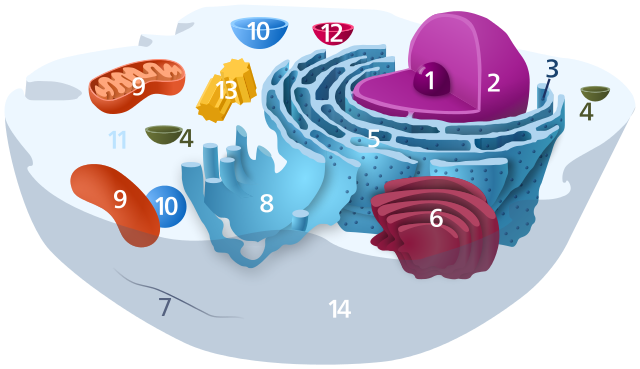
\includegraphics[width=\tmpwidth]{640px-Animal_Cell-svg.png} & % 
\onslide<4->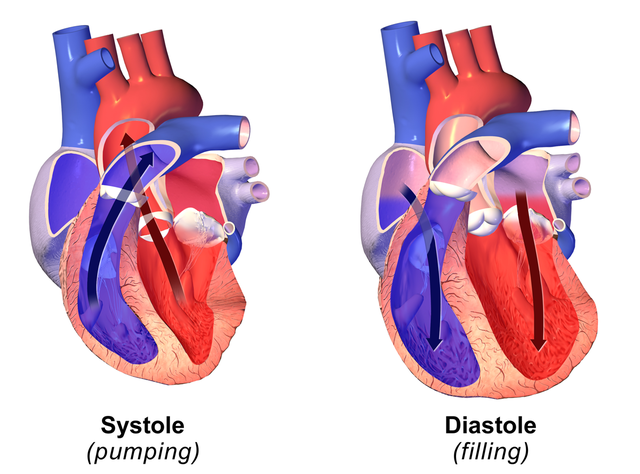
\includegraphics[width=\tmpwidth]{Systolevs_Diastole.png}
\end{tabular}
\end{table}

\end{frame}

\note[enumerate]{
\item Understanding genes means understanding biology
\item Far more than simply persuing knowledge, this means that we can actually
use this information towards 
}


% ------------------------------------------------------------------------------
\begin{frame}[label=geneontology]
\frametitle{The Gene Ontology Project}

\begin{figure}

\includegraphics[width=.5\linewidth]{go-logo.png}
\end{figure}

\begin{itemize}[<+->]
% \item Three domains: Cellular component, molecular function, biological process.
\item The GO project has $\sim$ 44,700 validated terms  \hyperlink{aphylo-goexample}{\beamergotobutton{more}}, $\sim$ 7.3M annotations on $\sim$ 4,500 species.
\item About $\sim$ 500,000 are on human genes.
\item Roughly half of human genes ($\sim$ 10,000 / 20,000) have some
form of annotation.
\item We know something of less than 10\% of known genes (near 1.7M).
\item An important effort of the GO has to do with phylogenetics...
\end{itemize}

\vfill
\hfill \textbf{source}: Statistics from \url{pantherdb.org} and \url{geneontology.org}

\end{frame}

\note[itemize]{
\item The Gene Ontology Project, which is an international scientific effort to develop
a knowledge base of biology from molecular level up to organism-level systems.
\begin{quote}
[\dots] develop an up-to-date, comprehensive, computational model of biological systems, from the molecular level to larger pathways, cellular and organism-level systems.
\item It has a large collection of genetic annotations from various types of evidence
including: experimentally, human curated information, and machine inferred.
\end{quote}

\item A long way since 1999 (20 years), there's still a lot to learn
\item This information has been crucial for biomedical research (e.g. translating
GWAS to treatment.)
}



% ------------------------------------------------------------------------------
\begin{frame}

\begin{figure}
\centering
{\footnotesize
\def\svgwidth{.7\linewidth}
\input{fig/Phylogenetic_tree-wiki.pdf_tex}
}
\caption{A phylogenetic tree of living things, based on RNA data and proposed by Carl Woese, showing the separation of bacteria, archaea, and eukaryotes (\href{https://en.wikipedia.org/wiki/File:Phylogenetic_tree.svg}{wiki})}
\end{figure}
\end{frame}

\note[enumerate]{
\item Phylogenetic trees show evolutionary relationships between species
\item Traditionally, we think about these based on say physical features, 
nowadays we build trees based on genetic distances between species.
}

% ------------------------------------------------------------------------------
\begin{frame}[t]
\frametitle{Phylogenetic Trees: The PANTHER classification system}
\begin{minipage}{.4\linewidth}
\pause\small
\begin{itemize}[<+->]
\item The PANTHER project (part of GO) provides information about evolutionary structure of 1.7 million
genes
\item These genes are grouped in 15,524 phylogenetic trees (families)
\item A single family can host multiple species
\end{itemize}
\end{minipage}
\hfill
\begin{minipage}{.5\linewidth}
\uncover<5->{
\begin{knitrout}
\definecolor{shadecolor}{rgb}{0.969, 0.969, 0.969}\color{fgcolor}\begin{figure}

{\centering 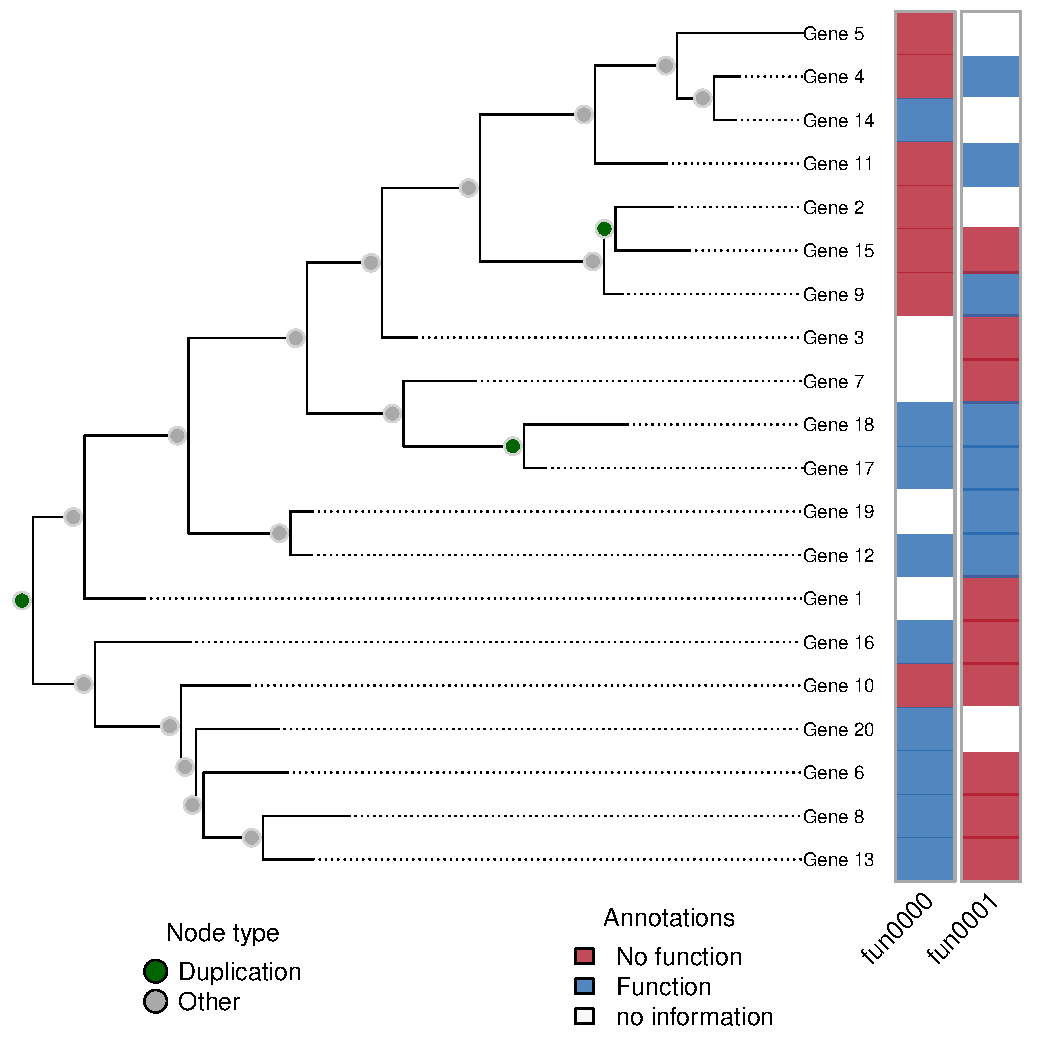
\includegraphics[width=.85\linewidth]{figure/random-tree-1} 

}

\caption[Simulated phylogenetic tree and gene annotations]{Simulated phylogenetic tree and gene annotations.}\label{fig:random-tree}
\end{figure}


\end{knitrout}
}
\end{minipage}
\end{frame}

\note[enumerate]{
\item Here we have an example of a (simulated) phylogenetic tree.
\item We will see this a couple of times during the presentation
\item This figure summarizes the information that I will be using
to infere gene functions:
\begin{itemize}
\item The tip nodes (leafs) are modern (known) genes
\item In general, The color bars next to each gene represent genetic annotations
(GO terms) in three different states: Has the function (blue), does not have the
function (red), and no information (white)
\item Each interior node represent ancestors which are classify as 
duplication/speciation/or horizontal transfer nodes
\item This is an hypothesis regarding to what type of event lead
to a split in the family.
\item we mostly care about whether these are duplication nodes not
since we believe that functional gain and loses are more likely
to happen at this stage.
\end{itemize}
}

%
\frame{
\centering
\Large
We can use \vspace{.5cm}

\textcolor{usccardinal}{ {\Huge evolutionary trees}} \vspace{.5cm}

to inform a model for predicting \vspace{.5cm}

 \textcolor{usccardinal}{{ \Huge genetic annotations!}}
}



\note[enumerate]{

There various approaches for this, some to highlight
\begin{itemize}%[<+->]
\item Text analysis like in \cite{Pesaranghader2016}
\item Protein-protein interaction networks like in \cite{Oliver2000,Piovesan2015}.
\item Phylogenetic based like SIFTER \cite{Engelhardt2005,Engelhardt2011}.
\begin{itemize}
\item Parameters to estimate: $2^{2P}$, where $P$ is the number of functions.
\end{itemize}
\end{itemize}

\vfill \hfill (a nice literature review in \cite{Jiang2016,Yu2018})

\item The last one being the most closely related to what we propose here
(details to be shown).
\item In SIFTER, functions are modeled using a transition matrix in
a Markov continuous model.
\item The main problem with this is that the computational complexity
of the model grows horribly (estimating a model with a 100 functions)
takes literally infinite time.
\item B/c of this, they truncate some of their modelling and work with
small sets of up to 5 functions in a single tree (for example).
\item One key point of most of these models is that these provide a
point estimate rather than a distribution, and mostly a binary
estimate of the annotation (yes/no).
}

% ------------------------------------------------------------------------------
\begin{frame}[label=aphylographicalview]
\frametitle{An evolutionary model of gene functions}

\definecolor{rootnode}{RGB}{0,159,211}
\definecolor{innernode}{RGB}{90,159,89}
\definecolor{leafnode}{RGB}{255,107,0}

\begin{minipage}{.48\linewidth}
\begin{itemize}
	\item<2-> \textcolor{rootnode}{Initial (spontaneous) gain of function}.
	\item<3-> \textcolor{innernode}{Loss/gain of offspring depends on: (a) the state of their parents ({\bf Markov process}), and (b) the type of node \hyperlink{duplicationvsspeciation}{\beamergotobutton{more}}}
	\item<4-> \textcolor{leafnode}{We control for human error.}
\end{itemize}
\end{minipage}
%
\begin{minipage}{.50\linewidth}
\begin{figure}
	\footnotesize
	\centering
	\def\svgwidth{.9\linewidth}
	\input{fig/aphylo.pdf_tex}
\end{figure}
\end{minipage}

\vspace{1.5cm}

\uncover<5->{We implemented the model using Felsenstein's' pruning algorithm (linear complexity) in the
R package \aphylopkg{} \hyperlink{aphylopkg}{\beamergotobutton{more}}.}

\vfill\hfill \hyperlink{other-models}{\beamergotobutton{other models}}
\hyperlink{aphyloalgorithmicview}{\beamergotobutton{other view}}

\end{frame}

\note[enumerate]{
\item In the version of the qual document you saw an implementation of the model
that did not incorporated information regarding the node types, but that is trivially
added by just adding a separate gain/loss parameter per type
\item Another venue we have explored is accounting for publicaction bias, most
annotations are of the positive type (has function), but few are (no function).
\item we have failed in the last tests.
\item The model has been throughly tested. In particular, we did a large scale
simulation study in which we used all 15,000 trees from panther to simulate
annotations and then fitted our model using MCMC to check for bias and coverage
probabilities (which are available in the paper)
\item The experiment was carriedout using USC's High Performance Computing
cluster with the R package slurmR (described in the document).
\item Now, I will show you more recent information in which we take 
data from PantherDB with GO annotations and fit a large pooled model.
}

% ------------------------------------------------------------------------------
\begin{frame}[t]
\frametitle{Prediction with real data}

\begin{minipage}{.39\linewidth}
\begin{table}[ht]
\centering
\scalebox{0.7}{
\begin{tabular}{ll*{2}{m{0.3\linewidth}<\centering}}
  \toprule
 & & \multicolumn{2}{c}{Prior} \\
 & & Uniform & Beta  \\ 
  \midrule
  \multicolumn{2}{l}{Mislab. prob.} \\
  & $\psi_0$ & 0.23 & 0.25 \\ 
  & $\psi_1$ & 0.01 & 0.01 \\ 
  \multicolumn{2}{l}{\textcolor<4->{usccardinal}{\textbf<4->{Gain/Loss at dupl.}}} \\
  & $\mu_{d0}$ & 0.97 & 0.96 \\ 
  & $\mu_{d1}$ & 0.52 & 0.58 \\ 
  \multicolumn{2}{l}{\textcolor<4->{usccardinal}{\textbf<4->{Gain/Loss at spec.}}} \\
  & $\mu_{s0}$ & 0.05 & 0.06 \\ 
  & $\mu_{s1}$ & 0.01 & 0.02 \\ 
  \multicolumn{2}{l}{Root node} \\
  & $\pi$ & 0.81 & 0.45  \\ 
\midrule 
\multicolumn{2}{l}{Leave-one-out AUC} \\
  & Mean & 0.69 & 0.67 \\
  & Median & 0.81 & 0.75 \\
   \bottomrule
\end{tabular}
}
\caption{Parameter estimates using different priors.} 
\end{table}
%
\end{minipage}
\begin{minipage}{.59\linewidth}
\begin{itemize}[<+->]
\item 141 pooled functions (trees) with 7,388 genes with 0/1 annotations.
\item Parameter estimates are actually probabilities.
\item Data driven results (uninformative prior).
\item \textcolor{usccardinal}{Biologically meaningful results.}
\item Took about 5 minutes each.
\end{itemize}
\end{minipage}

\end{frame}

\note[enumerate]{
\item The data used here corresponds to a subset of the trees.
\item Right now, the main criteria was: (1) must have at least one annotation
of each type, and (2) must not have large sets of siblings (this due to
numerical underflow issues, WIP)
}

% % ------------------------------------------------------------------------------
% \begin{frame}
% \frametitle{Paper 1: Pooled estimation (worth it?)}
% 
% \begin{figure}
% \centering
% 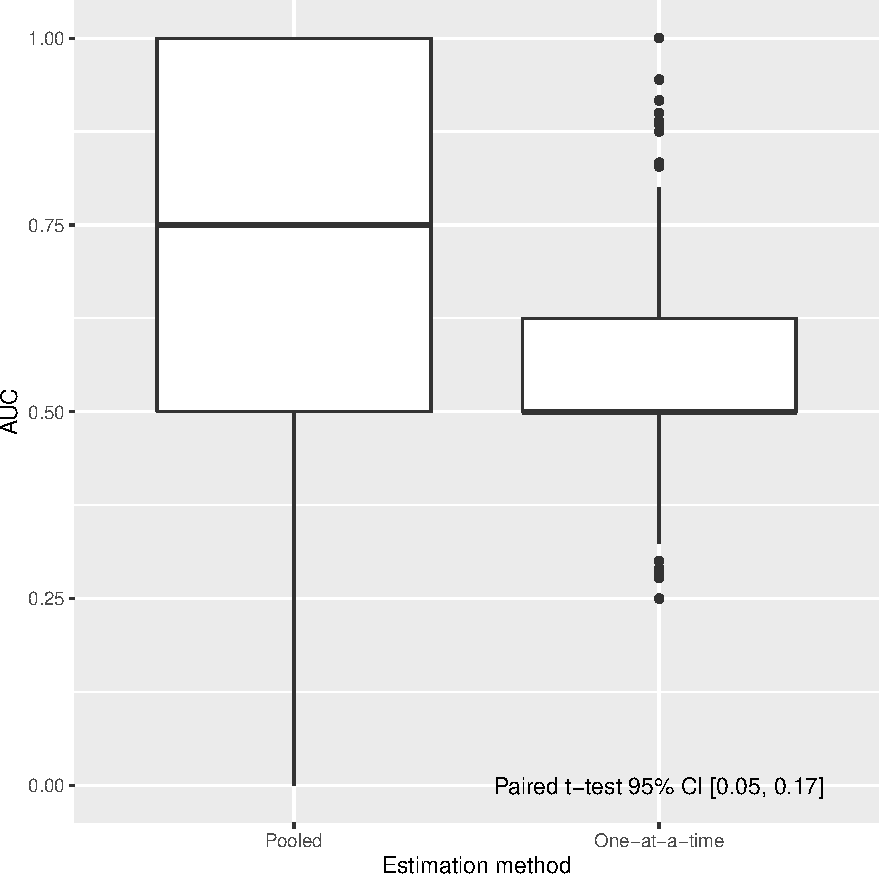
\includegraphics[width=.5\linewidth]{comparing-accuracy-1.pdf}
% \end{figure}
% 
% \end{frame}

% ------------------------------------------------------------------------------
\begin{frame}
\frametitle{Prediction with real data: Leave-one-out}

\begin{figure}
\centering
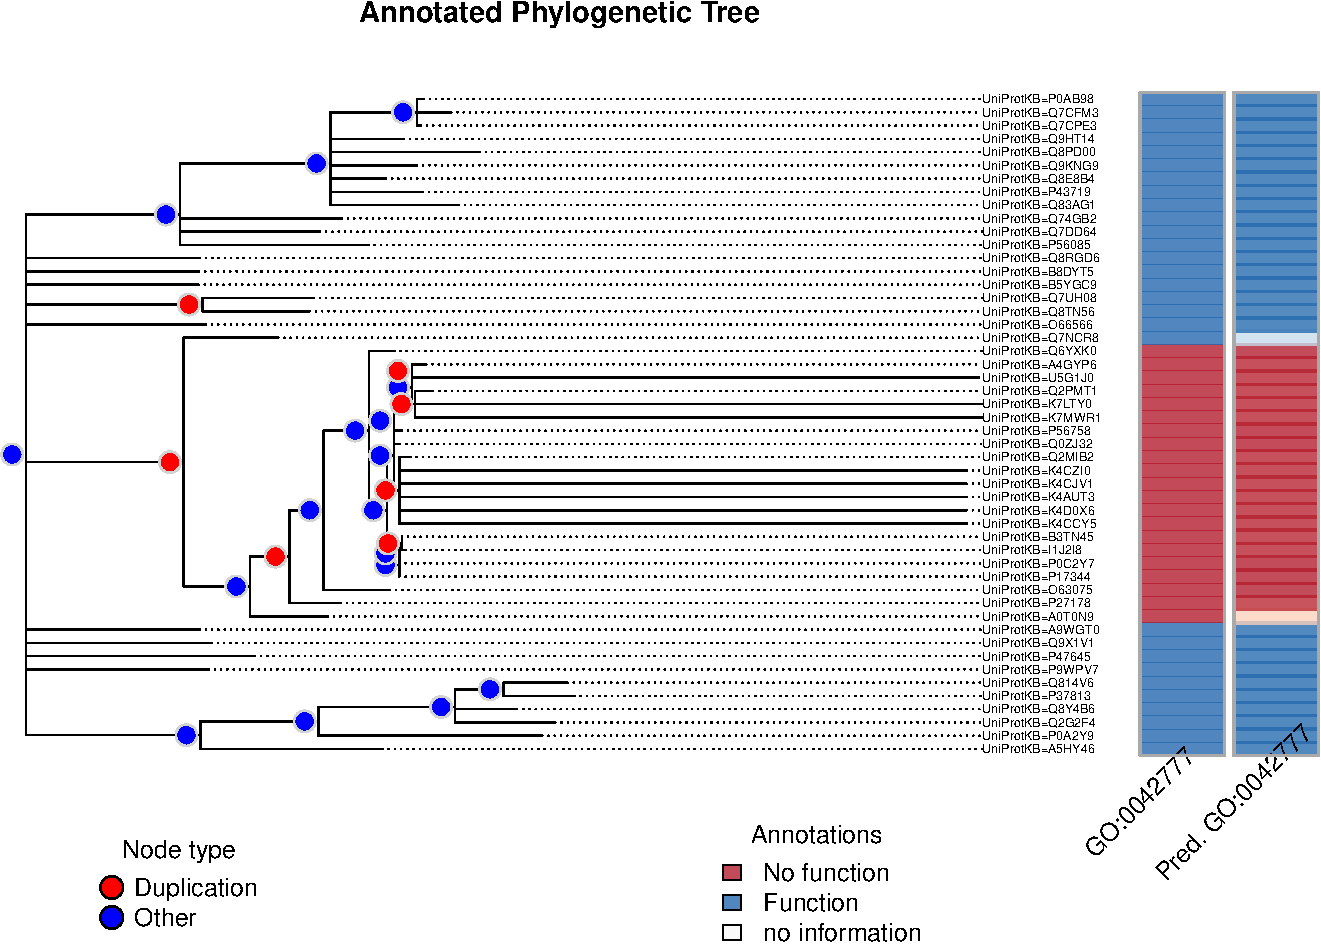
\includegraphics[width=.7\linewidth]{annotations1.pdf}
\end{figure}

\end{frame}

% ------------------------------------------------------------------------------
\begin{frame}
\frametitle{Prediction with real data: Out-of-sample prediction}

\begin{figure}
\centering
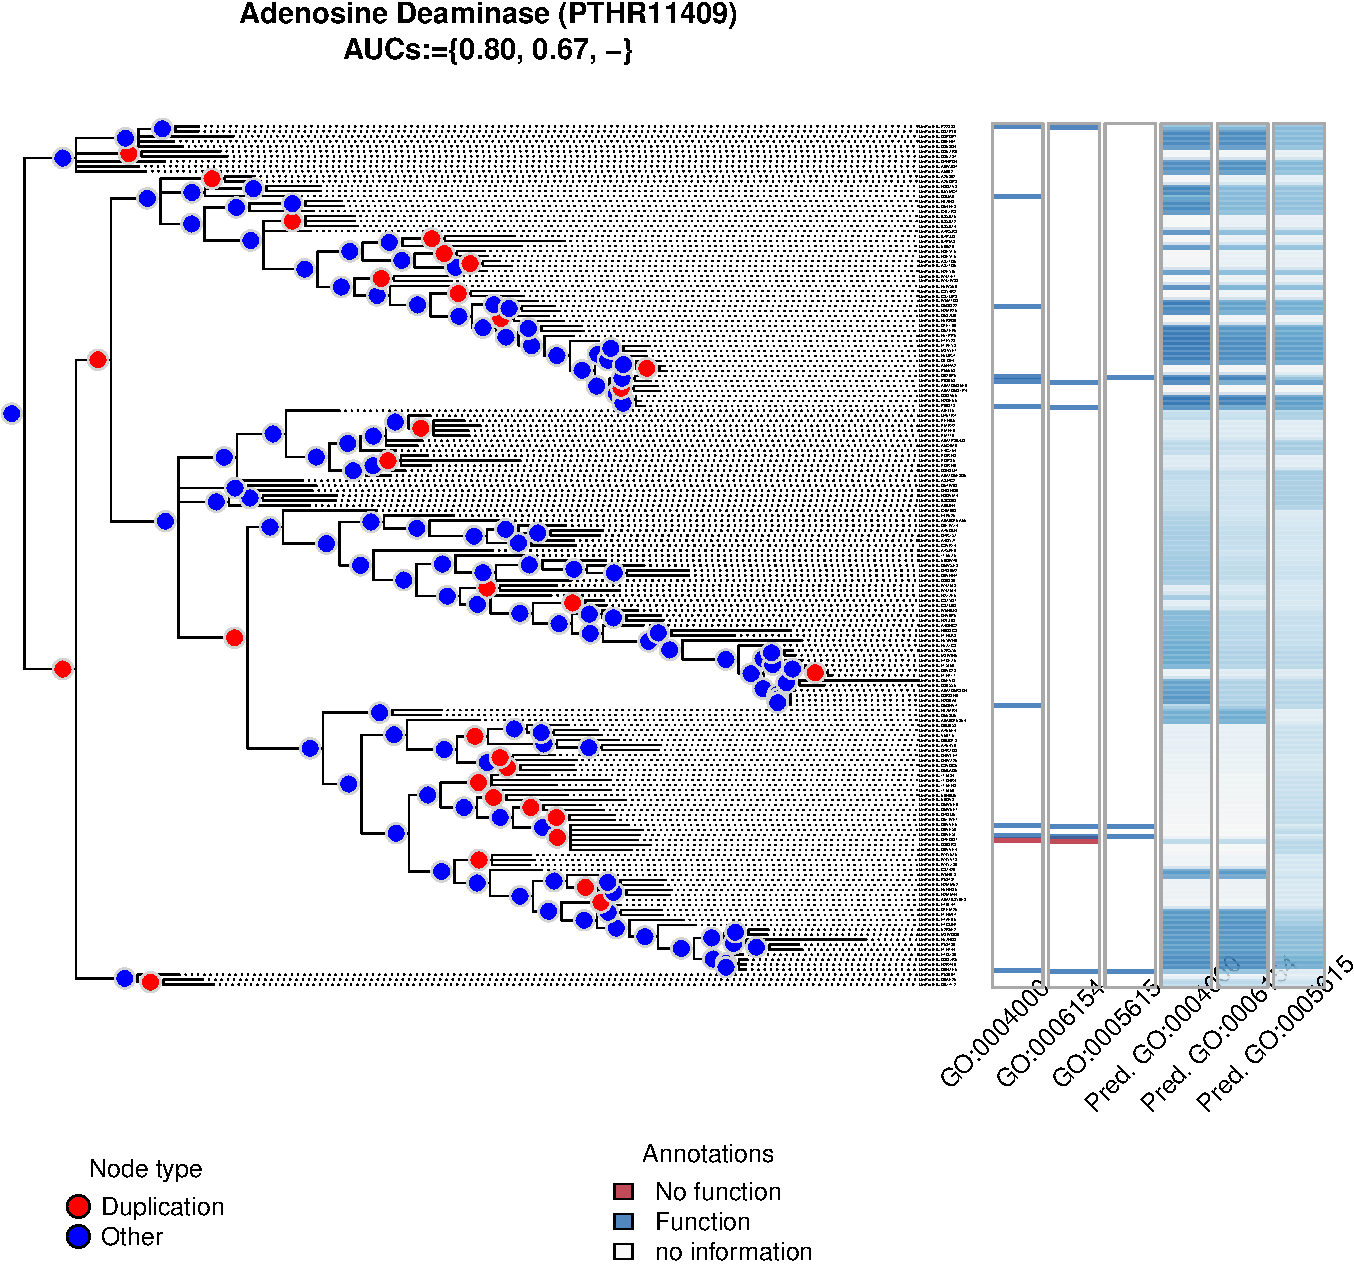
\includegraphics[width=.65\linewidth]{out-of-sample1-1.pdf}
\end{figure}

\end{frame}

% ------------------------------------------------------------------------------
\begin{frame}[t]
\frametitle{Paper 1: On the prediction of gene functions using phylogenetic trees}

{\bf \large Key takeaways}
\begin{beamercolorbox}[dp=1ex]{conclusions}
\begin{itemize}
\item A parsimonious model for predicting gene functions using phylogenetics.
\item Computationally scalable. SIFTER (our benchmark)
would take about 66 years (yes, years) to estimate a model for 100 families
of size 300, we take about 5 minutes.
\item Meaningful biological results.
\item Preliminary accuracy results comparable to state-of-the-art phylo-based models.
\end{itemize}
\end{beamercolorbox}\pause

{\bf \large Challenges}
\begin{beamercolorbox}[dp=1ex]{conclusions}
\begin{itemize}
\item Offspring are conditional independent on their parent and\pause{}
\item Functions evolve independently. \hyperlink{duplicationvsspeciation}{\beamergotobutton{more}}
\end{itemize}
\end{beamercolorbox}

\end{frame}



% ------------------------------------------------------------------------------
\section{Paper 2: Exponential Random Graph Models for Small Networks}
% \frame{\frametitle{Contents}\tableofcontents}

\begin{frame}[t]
\usebeamertemplate{section intro}{}{}
\textcolor{uscgold}{
\Large {\bf Exponential Random Graph Models for Small Networks} \vskip0.25em
\large \textit{Joint with}: Andrew Slaughter and Kayla de la Haye
}
\end{frame}

\begin{frame}
\frametitle{What are Exponential Random Graph Models}

Exponential Family Random Graph Models, aka \alert{ERGMs} are:\pause

\begin{itemize}[<+->]
\item Statistical models of (social) networks
\item In simple terms: statistical inference on what network patterns/structures/motifs
govern social networks
\begin{figure}
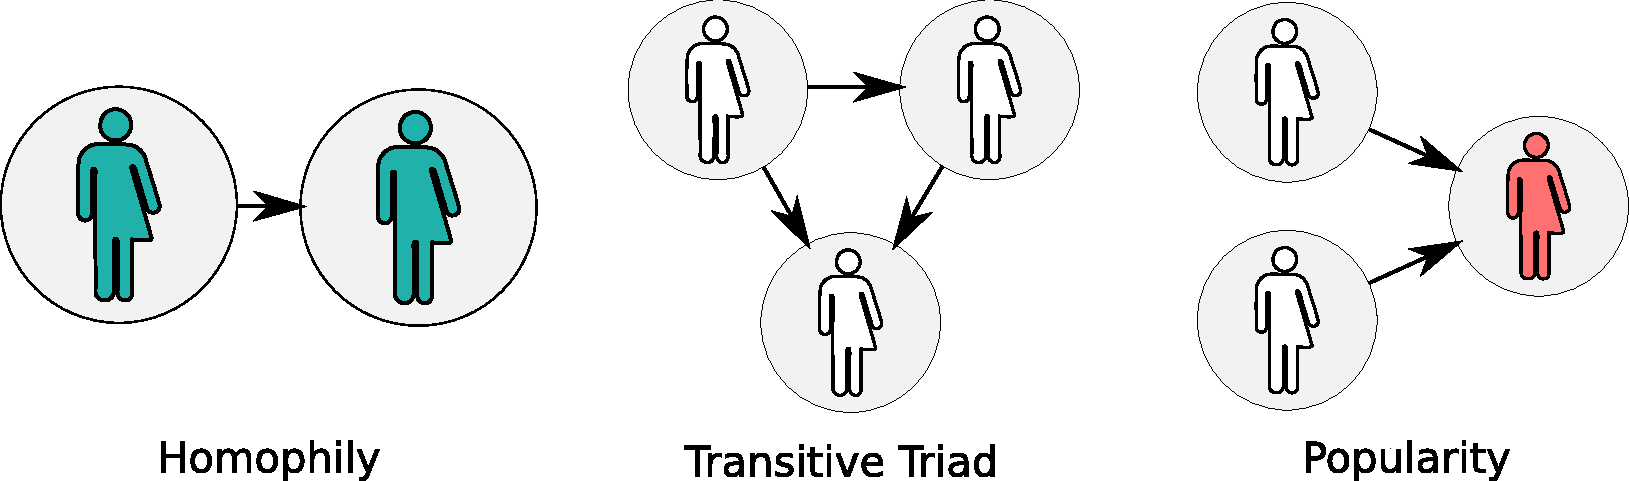
\includegraphics[width=.6\linewidth]{friendly-terms.pdf}
\end{figure}
\end{itemize}

\end{frame}

% ------------------------------------------------------------------------------
\begin{frame}[label=ergmeq]
\frametitle{ERGMs (cont'd)}
\begin{figure}
\centering
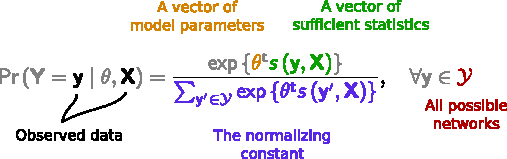
\includegraphics[width=.7\linewidth]{parts-of-ergm.pdf}
\end{figure}

\uncover<2->{The normalizing constant has $2^{n(n-1)}$ terms!}

% \vfill\hfill \hyperlink{ergmterms}{\beamergotobutton{more on terms}}
\end{frame}

% ------------------------------------------------------------------------------
\begin{frame}[label=ergmterms]

{\bf\color{suffstat} Sufficient statistics} have various forms

\def\fig1width{.45\linewidth}
\begin{figure}[tb]
\centering
\begin{tabular}{m{.2\linewidth}<\centering m{.4\linewidth}<\raggedright}
\toprule Representation & Description  \\ \midrule

\includegraphics[width=\fig1width]{ergm-terms/mutual.pdf} & Mutual Ties (Reciprocity)\linebreak[4]$\sum_{i\neq j}y_{ij}y_{ji}$  \\
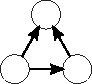
\includegraphics[width=\fig1width]{ergm-terms/ttriad.pdf} & Transitive Triad (Balance)\linebreak[4]$\sum_{i\neq j\neq k}y_{ij}y_{jk}y_{ik}$  \\

\includegraphics[width=\fig1width]{ergm-terms/homophily.pdf} & Homophily\linebreak[4]$\sum_{i\neq j}y_{ij}\mathbf{1}\left(x_i=x_j\right)$ \\
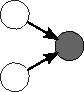
\includegraphics[width=\fig1width]{ergm-terms/nodeicov.pdf} & Covariate Effect for Incoming Ties\linebreak[4]$\sum_{i\neq j}y_{ij}x_j$ \\
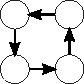
\includegraphics[width=\fig1width]{ergm-terms/fourcycle.pdf} & Four Cycle\linebreak[4]$\sum_{i\neq j \neq k \neq l}y_{ij}y_{jk}y_{kl}y_{li}$  \\
\bottomrule
\end{tabular}
\end{figure}

% \vfill\hfill \hyperlink{ergmeq}{\beamerreturnbutton{go back}}
\end{frame}

% -----------------------------------------------------------------------------
\begin{frame}[label=ergm-toyexample]

\begin{columns}[c]

\begin{column}[c]{.4\linewidth}

In this network\linebreak

\begin{knitrout}
\definecolor{shadecolor}{rgb}{0.969, 0.969, 0.969}\color{fgcolor}

{\centering 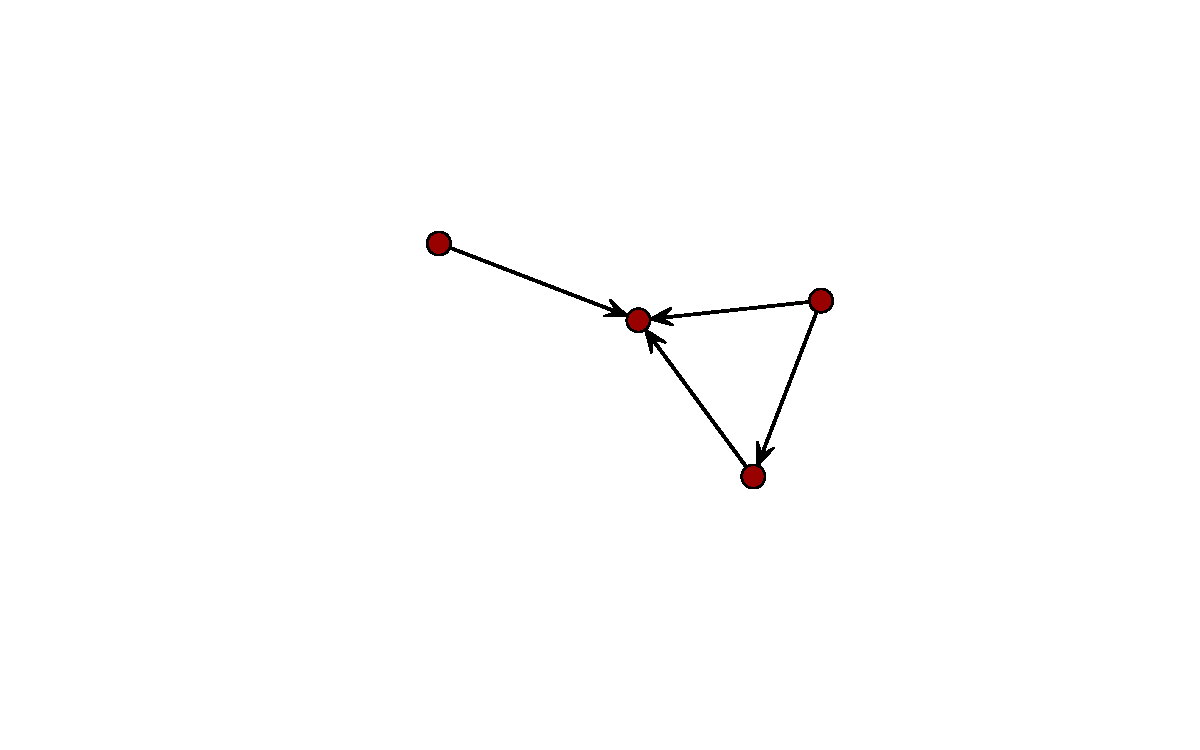
\includegraphics[width=.9\linewidth]{figure/simple-model-1} 

}



\end{knitrout}

\pause

We see 4 \textbf{edges}, 1 \textbf{transitive triad} and \textbf{no mutual ties}.

\end{column}

\pause

\begin{column}[c]{.4\linewidth}

The probability function of this model would be

\footnotesize

\begin{equation*}
\Prcond{\Graph = \graph}{\theta} = \frac{\exp{4\theta_{edges} + \theta_{ttriads} \textcolor{lightgray}{+ 0\theta_{mutual}}}}{%
\sum_{\graph'\in\GRAPH} \exp{\transpose{\theta} \sufstats{\graph'}}}
\end{equation*}

\normalsize

\noindent with $\theta = \transpose{[\theta_{edges}\quad \theta_{ttriads} \quad \theta_{mutual}]}$

\end{column}

\end{columns}



\pause

\vspace{1cm}

This model has \textbf{MLE parameter estimates} of -0.20 (low density), 0.28 (high chance of ttriads), and -Inf (low chance of mutuality) for the parameters \texttt{edges}, \texttt{ttriads}, and \texttt{mutual} respectively.

\end{frame}

% ------------------------------------------------------------------------------
\begin{frame}[label=art]
\frametitle{ERGMs: State of the Art}
\pause
Medium-large (dozens to a couple of thousand vertices) networks

\begin{itemize}
\item Markov Chain Monte Carlo (MCMC) based approaches like MC-MLE or Robbins-Monro Stochastic Approximation. \hyperlink{mcmle}{\beamergotobutton{details}}
\item Maximum Pseudo Likelihood (MPLE)
\end{itemize}\pause

large-huge networks (up to millions of vertices)

\begin{itemize}
\item Parametric bootstrap
\item Conditional joint estimation (like snowball sampling, a.k.a. divide and conquer)
\item Equilibrium Expectation Algorithm (millions of vertices)
\end{itemize}\pause

All of these methods are approximations!

\end{frame}

% ------------------------------------------------------------------------------
\begin{frame}[c]
\frametitle{Do we care about small networks?}

\begin{minipage}{.40\linewidth}
We see small networks everywhere\pause

\begin{itemize}[<+->]
\item Families and friends
\item Small teams
\item Egocentric networks
\item Online networks (sometimes)
\item etc.
\end{itemize}
\end{minipage}
\hfill
\uncover<7->{
\begin{minipage}{.55\linewidth}
\centering\large
Small networks come in samples
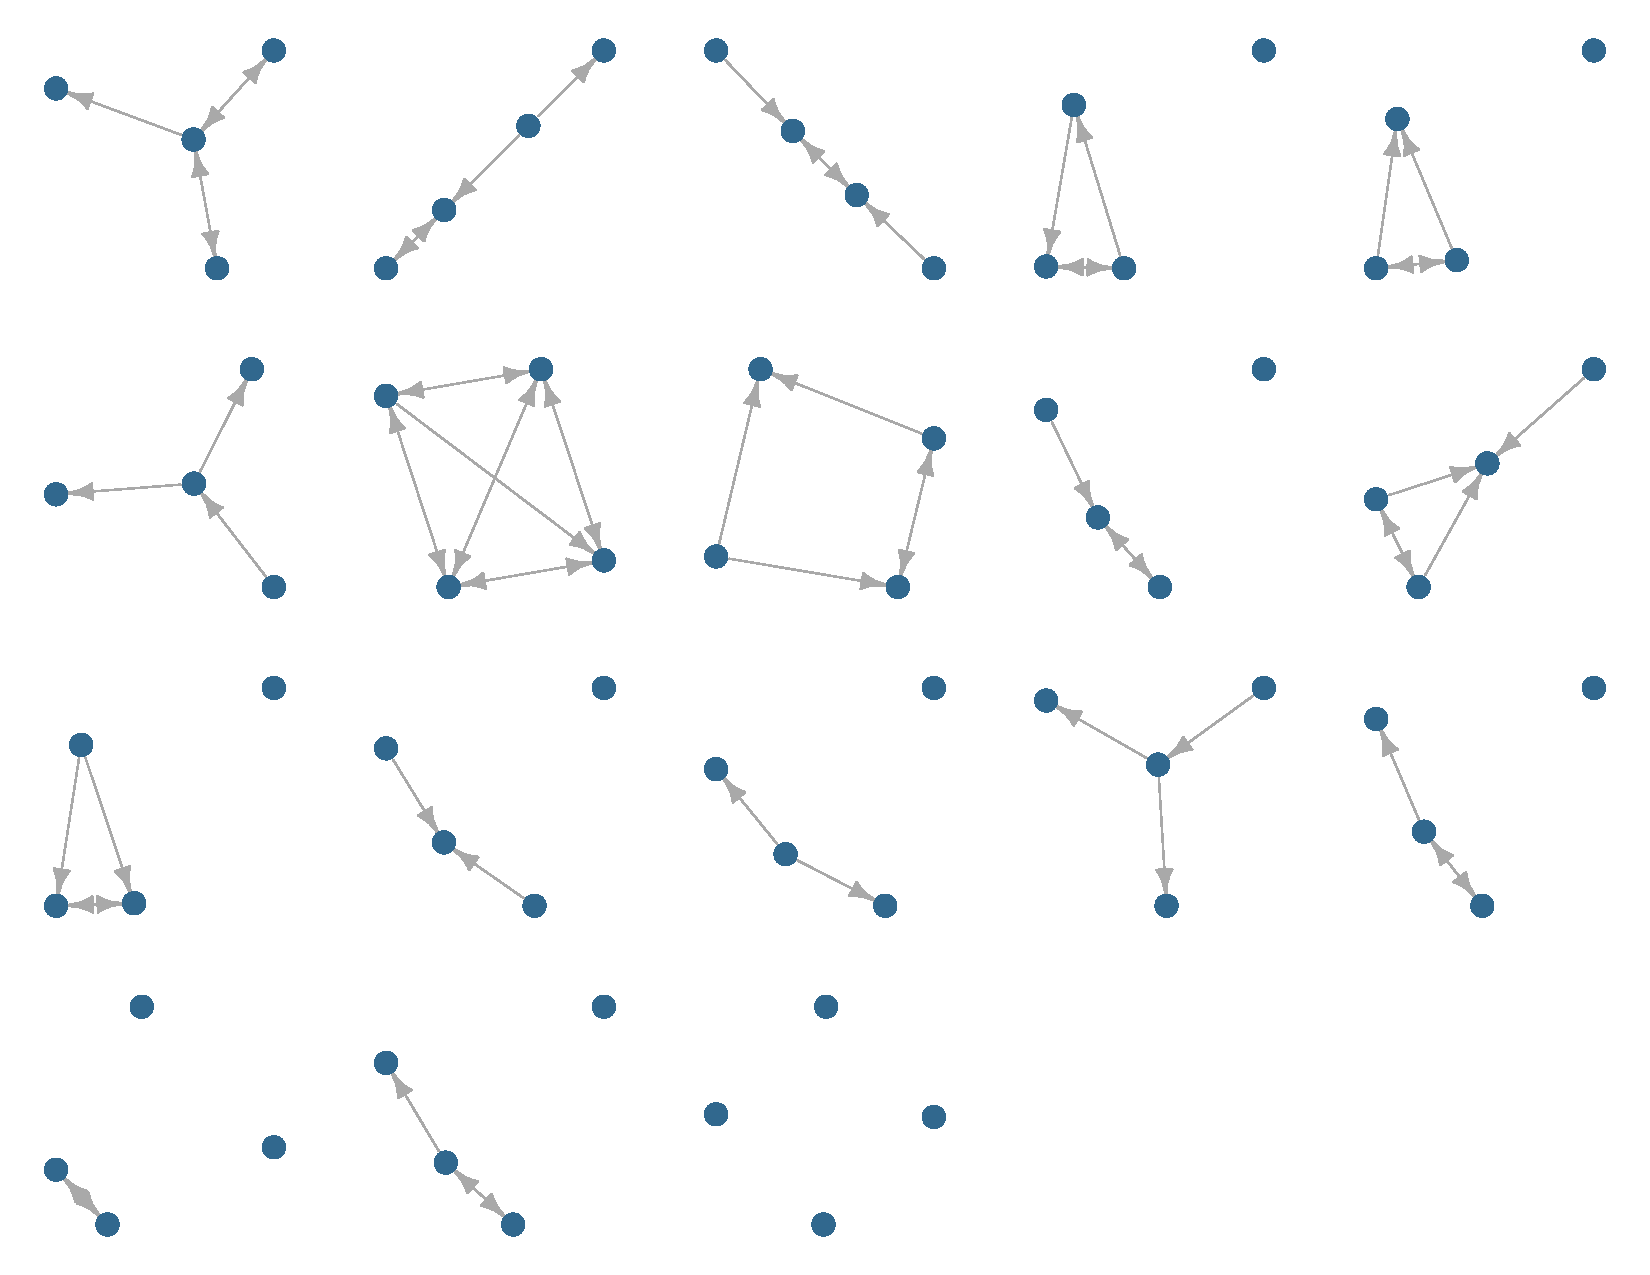
\includegraphics[width=.85\linewidth]{plot-graph-4-1.pdf}
% 
\includegraphics[width=.95\linewidth]{american-chopper-argument-ergmitos.png}
\end{minipage}
}
\end{frame}

% % ------------------------------------------------------------------------------
% \begin{frame}
% \frametitle{ERGMs for Small Networks}
% 
% From the methodological point of view, current methods are great, but:\pause
% 
% \begin{itemize}
% \item Possible accuracy issues (error rates)\pause
% \item Prone to degeneracy problems (sampling and existence of MLE)\pause
% \item It is not MLE...
% \end{itemize}
% 
% \end{frame}

% ------------------------------------------------------------------------------
\begin{frame}[label=ergmito]
\frametitle{ERGMs for Small Networks}

\uncover<4->{
\begin{figure}
\centering
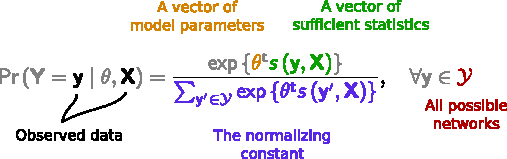
\includegraphics[width=.5\linewidth]{parts-of-ergm.pdf}
\end{figure}
}

\begin{itemize}[<+->]

\item In the case of small-enough networks, computation of the likelihood becomes
computationally feasible.

\item This allow us to directly compute {\bf\color{normconst} the normalizing constant}.\pause

\item Using the exact likelihood opens a huge window of methodological-possibilities.

\item We implemented this and more in the \ergmitopkg{} R package \hyperlink{ergmitopkg}{\beamergotobutton{more}}
\end{itemize}


\end{frame}


%-

\begin{frame}
Sidetrack...\vspace{.5cm}

\begin{minipage}[c]{1\linewidth}
\large \textbf{ito, ita}: From the latin -\textit{\=ittus}. suffix in Spanish used to denote small or affection. e.g.:

\hspace{.5cm} \textit{¡Qué lindo ese perr\textcolor{USCCardinal}{\textbf{ito}}!} / \textit{What a beautiful little dog!}

\hspace{.5cm} \textit{¿Me darías una tac\textcolor{USCCardinal}{\textbf{ita}} de azúcar?} / \textit{Would you give me a small cup of sugar?}
\normalsize
\end{minipage}\pause

% Screen shot of ERGMito tweet.
\vfill

\alert{Special thanks to George Barnett who proposed the name during the 2018 NASN!}

\end{frame}

% ------------------------------------------------------------------------------
\begin{frame}[label = ergmitoexample]
\frametitle{\ergmitopkg{} example}

\begin{minipage}{.4\linewidth}
\begin{figure}
\centering
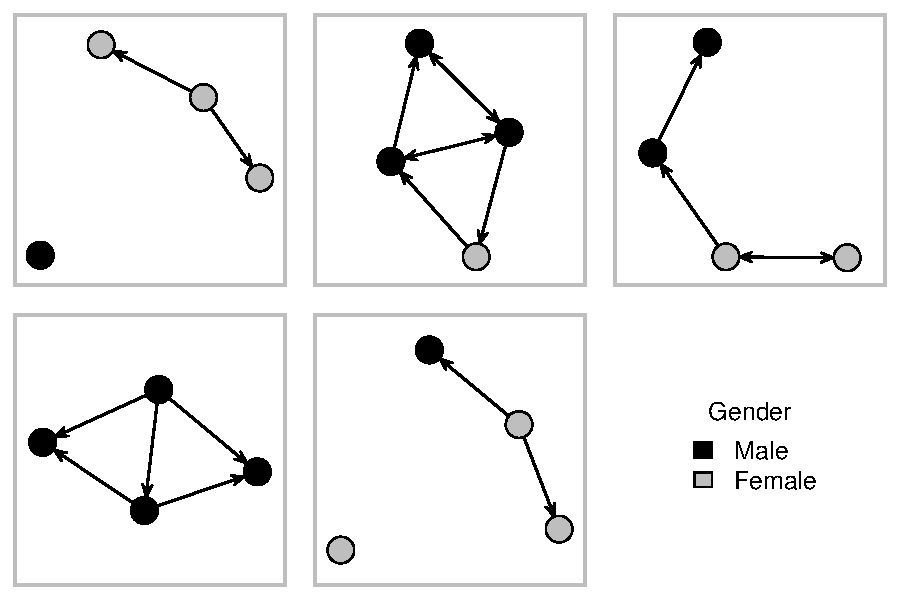
\includegraphics[width = .9\linewidth]{fivenets_graphs.pdf}
\caption{Random sample of 5 networks simulated using the ergmito package}
\end{figure}
\end{minipage}
\hfill
\begin{minipage}{.55\linewidth}
\pause
\footnotesize
\begin{table}
\begin{tabular}{l*{2}{m{.2\linewidth}<\centering}}
\hline
 & Bernoulli & Full model \\
\hline
Edge-count             & $-0.69^{*}$ & $-1.70^{**}$ \\
                      & $(0.27)$    & $(0.54)$     \\
Homophily (on Gender) & & $1.59^{*}$   \\
                      & & $(0.64)$     \\
\hline
AIC                   & 78.38       & 73.34        \\
BIC                   & 80.48       & 77.53        \\
Log Likelihood        & -38.19      & -34.67       \\
Num. networks         & 5           & 5            \\
\hline
\multicolumn{3}{l}{\scriptsize{Standard errors in parenthesis. $^{***}p<0.001$, $^{**}p<0.01$, $^*p<0.05$}}
\end{tabular}
\caption{Fitted ERGMitos using the fivenets dataset.}
\label{table:coefficients}
\end{table}
\normalsize
\end{minipage}\pause

We performed a large simulation study \hyperlink{ergmitodgp}{\beamergotobutton{more}}
comparing MC-MLE (ergm) with MLE (ergmito).

\end{frame}

% ------------------------------------------------------------------------------
\begin{frame}[label=ergmsims,allowframebreaks]
\frametitle{Paper 2 Simulation Studies: Error rate}

\begin{minipage}{.45\linewidth}
\begin{itemize}[<+->]
\item The MC-MLE implementation failed $\sim$ 5,000/20,000 times
\item In $\sim$700 of those cases ergmito (MLE) reported a significant effect
\item I no case that MLE failed MC-MLE reported an effect.
\end{itemize}
\end{minipage}
\hfill
\begin{minipage}{.45\linewidth}
\begin{figure}
\centering
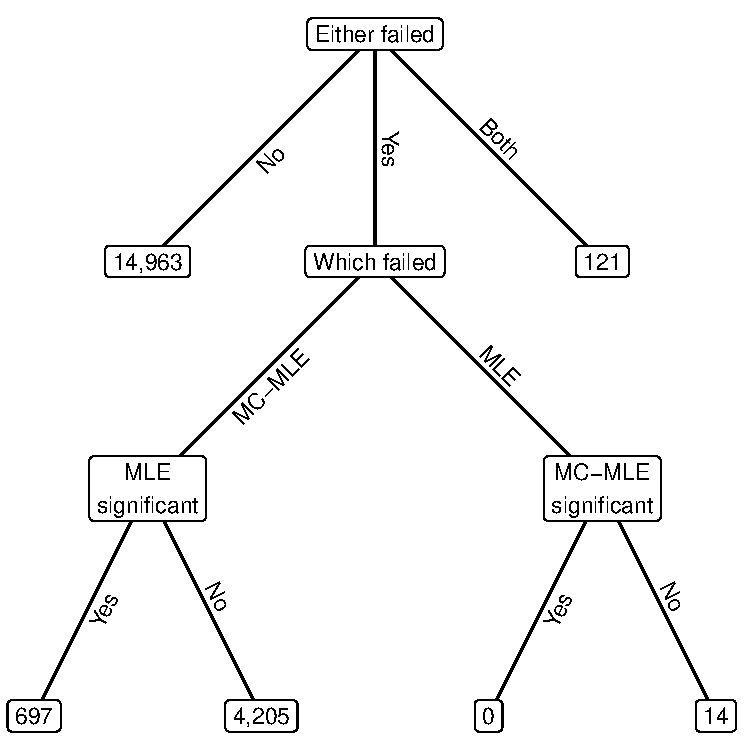
\includegraphics[width=.9\linewidth]{failed-tree.pdf}
\end{figure}
\end{minipage}

% \hyperlink{ergmitoexperiment}{\beamerreturnbutton{go back}}

\end{frame}

% ------------------------------------------------------------------------------
\begin{frame}
\frametitle{Paper 2 Simulation Studies: Empirical Type I error}

\footnotesize

\begin{table}[ht]
	\centering
	\begin{tabular}{cccc}
		\toprule & \multicolumn{2}{c}{P(Type I error)} \\ \cmidrule(r){2-3}
		Sample size  & \makecell{MC-MLE \\ (\ergmpkg{})} & \makecell{MLE \\ (\ergmitopkg{})} & $\chi^2$ \\ 
		\midrule
		5 & 0.084 & 0.057 & 11.71 *** \\ 
		10 & 0.070 & 0.045 & 12.46 *** \\ 
		15 & 0.084 & 0.066 & 5.55 * \\ 
		20 & 0.074 & 0.060 & 3.58  \\ 
		30 & 0.057 & 0.052 & 0.67  \\ 
		50 & 0.046 & 0.044 & 0.17  \\ 
		100 & 0.048 & 0.048 & 0.00  \\ 
		\bottomrule
	\end{tabular}
	\caption{\label{tab:typeI}Empirical Type I error rates. The $\chi^2$ statistic is from a 2-sample test for equality of proportions, and the significance levels are given by *** $p < 0.001$, ** $p < 0.01$, and * $p < 0.05$.} 
\end{table}

\end{frame}

% ------------------------------------------------------------------------------
\begin{frame}[label=ergmitoexperiment]
\frametitle{Paper 2 Simulation Studies: Elapsed time}

\begin{figure}
\centering
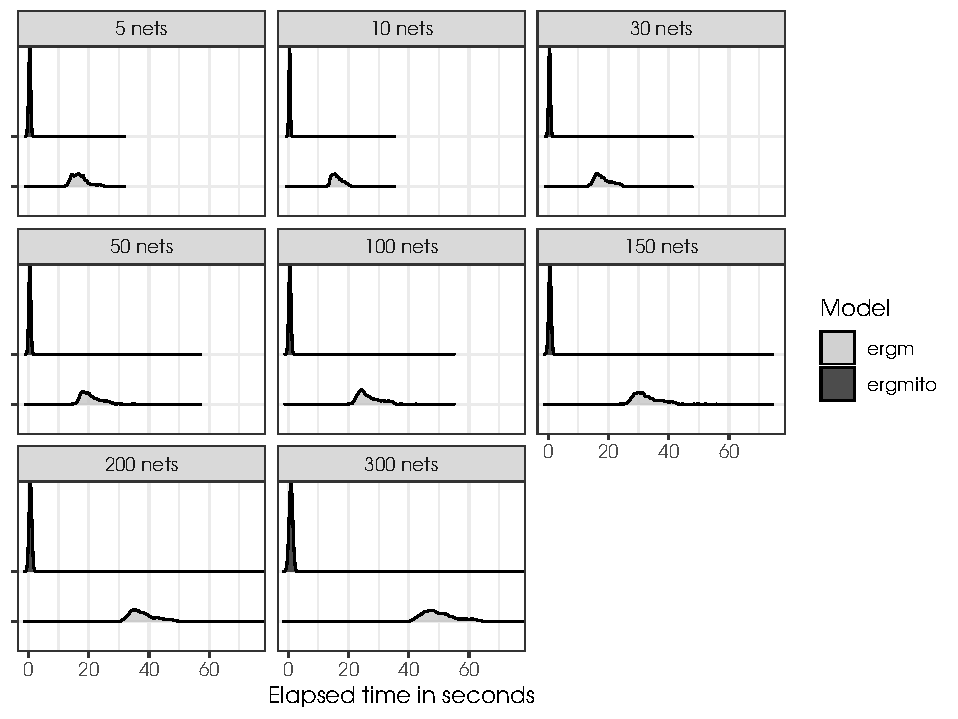
\includegraphics[width=.6\linewidth]{bias-elapsed-02-various-sizes-4-5-ttriad.pdf}
\end{figure}

\vfill\hfill\hyperlink{ergmito-bias}{\beamergotobutton{more results}}

\end{frame}

% ------------------------------------------------------------------------------
\begin{frame}
\frametitle{Paper 2: Exponential Random Graph Models for Small Networks}

{\bf \large Key takeaways}
\setbeamercolor{conclusions}{bg=usclightgray!60!white, fg=uscdarkgray}
\begin{beamercolorbox}[dp=1ex]{conclusions}
\begin{itemize}
\item New extension of ERGMs using exact statistics for small networks
(families, teams, etc.)
\item Performance: Same (un)bias, Lower Type I error rates, (way) faster.
\item Opens the door the new methods, e.g. Mixed effects, LRT, etc.
\end{itemize}
\end{beamercolorbox}

\vfill\pause

{\bf \large Challenges}
\begin{beamercolorbox}[dp=1ex]{conclusions}
\begin{itemize}
\item Computationally, we can do better in terms of speed/memory.\pause
\item Have a good way of assessing goodness-of-fit.\pause
\item Explore extending this method for (very) large networks.
\end{itemize}
\end{beamercolorbox}

\end{frame}

% ------------------------------------------------------------------------------
% ------------------------------------------------------------------------------
% ------------------------------------------------------------------------------
% ------------------------------------------------------------------------------
\section{Future Research}

\begin{frame}[c]
\usebeamertemplate{section intro}{}{}
\textcolor{uscgold}{
\Large {\bf Future Research}
}
\end{frame}

% ------------------------------------------------------------------------------
\begin{frame}[t]
\frametitle{Future Research: phylogenetic models}

\begin{itemize}
\item Make the model hierarchical when pooling trees\pause
\begin{itemize}
\item Different mutation rates per class of tree/function
\item Can be complicated to fit (how many classes?)
\end{itemize}\pause
\item Use a framework similar to Exponential Random Graph Models:\pause
\begin{itemize}
\item A generalization of the model
\item Extends to account for joint dist of functions+siblings
\item Can incorporate aditional information such as branch lenghts
\item Yet computationally more compact compared to SIFTER (iso-statistics)
\end{itemize}
\end{itemize}
\pause
$$
\Prcond{\Ann=\{\ann{n1}, \ann{n2},\dots\}}{\ann{\parent{n1, \dots}}} = \frac{\exp{\mu^{T} s(\mathbf{x}|\ann{\parent{\cdot}})}}{\sum_{\mathbf{x}'}\exp{\mu^{T} s(\mathbf{x}'|\ann{\parent{\cdot}})}}
$$


\end{frame}

% % ------------------------------------------------------------------------------
% \begin{frame}[t]
% \frametitle{Future Research: phylogenetic models}
% 
% \textbf{Example 1}\pause
% \begin{itemize}[<+->]
% \item 2 siblings 2 function involves modelling the following array:
% 
% $$
% \left[\begin{array}{c}x_{p1}\\x_{p2}\end{array}\right] \to
% \left(%
% \left[\begin{array}{c} x_{i1} \\ x_{i2}\end{array}\right],%
% \left[\begin{array}{c} x_{j1} \\ x_{j2}\end{array}\right]
% \right)
% $$
% \item Here we have $2^2 = 4$ possible states.
% \end{itemize}
% 
% \only<4->{\textbf{Example 2}}
% 
% \begin{itemize}[<+->]
% \item If we treat siblings independent, but work with 5 functions, SIFTER needs
% to estimate $2^{10} = 1,024$ parameters.
% 
% \item Our approach can reduce this number to, for example, 11 terms:
% \begin{itemize}
% \item $5\times 4 / 2 = 10$ statistics for pairwise correlation.
% \item One statistic accounting for longest branch.
% \end{itemize}
% \end{itemize}
% 
% \end{frame}

% ------------------------------------------------------------------------------
\begin{frame}[t]
\frametitle{Future Research: phylogenetic models}

Imagine that we have 3 functions (rows) and that each node has 2 siblings (columns)

\mode<beamer>{
  \begin{table}
  \begin{tabular}{llcc}
  \toprule
  & & \multicolumn{2}{c}{\bf Transitions to} \\
   & & Case 1 & Case 2 \\ \cmidrule(r){3-4}
  \multicolumn{2}{r}{\textbf{Parent} $\begin{array}{c}\mbox{A} \\ \mbox{B} \\ \mbox{C}\end{array}\left[\begin{array}{c}0 \\ 1 \\ 0\end{array}\right]$} & 
  $\left[\begin{array}{cc} %
    0 & \nhlc{1-3}{0}\hlc{4}{0}\nhlc{5-}{0} \\ %
    1 & \nhlc{1-3}{0}\hlc{4-5}{0}\nhlc{6-}{0} \\ %
    0 & \nhlc{1-2}{1}\hlc{3-5}{1}\nhlc{6-}{1} %
    \end{array}\right]$ & 
  $\left[\begin{array}{cc} %
    \nhlc{-2}{1}\hlc{3}{1}\nhlc{4}{1}\hlc{5}{1}\nhlc{6-}{1} & 0 \\ %
    \nhlc{1-4}{0}\hlc{5}{0}\nhlc{6-}{0} & \nhlc{1-4}{0}\hlc{5}{0}\nhlc{6-}{0} \\ %
    \nhlc{-2}{1}\hlc{3}{1}\nhlc{4}{1}\hlc{5}{1}\nhlc{6-}{1} & 0 %
    \end{array}\right]$ \pause \\ \midrule 
  \multicolumn{3}{l}{\textbf{Sufficient statistics}} \pause \\ 
  & \# Gains & 1 & 2 \pause \\
  & \# only one offspring changes & 1 & 0 \pause \\
  & \# Swaps (0$\to$1, 1$\to$0) & 2 & 4 \\ \bottomrule
  \end{tabular}
  \end{table}
}
\mode<handout>{
  \begin{table}
  \begin{tabular}{llcc}
  \toprule
  & & \multicolumn{2}{c}{\bf Transitions to} \\
   & & Case 1 & Case 2 \\ \cmidrule(r){3-4}
  \multicolumn{2}{r}{\textbf{Parent} $\begin{array}{c}\mbox{A} \\ \mbox{B} \\ \mbox{C}\end{array}\left[\begin{array}{c}0 \\ 1 \\ 0\end{array}\right]$} & 
  $\left[\begin{array}{cc} %
    0 & 0 \\ %
    1 & 0 \\ %
    0 & 1 %
    \end{array}\right]$ & 
  $\left[\begin{array}{cc} %
    1 & 0 \\ %
    0 & 0 \\ %
    1 & 0 %
    \end{array}\right]$ \pause \\ \midrule 
  \multicolumn{3}{l}{\textbf{Sufficient statistics}} \pause \\ 
  & \# Gains & 1 & 2 \pause \\
  & \# only one offspring changes & 1 & 0 \pause \\
  & \# Swaps (0$\to$1, 1$\to$0) & 2 & 4 \\ \bottomrule
  \end{tabular}
  \end{table}
}

\pause
In SIFTER, for modelling 3 functions, we need $2^{2\times 3} = 64$ parameters.

\end{frame}

% ------------------------------------------------------------------------------
\begin{frame}[t]
\frametitle{Future Research: ERGMitos}

{\bf Goodness-of-fit}\pause
\begin{itemize}
\item Is something that will need to be addressed at some point.\pause
\item The problem is not easy as we need to deal a discrete distribution.\pause
\item Two key questions: What sufficient statistic to look at? what test?
\end{itemize}

\pause {\bf ERGMs for large networks} \pause
\begin{itemize}
\item There is still no standard way to estimate ERGMs for large networks.\pause
\item Most atempts are still depending on simulation methods.\pause
\item We could use the Snowball Sampling framework together with ERGMitos.\pause{}
(... I would call this ERGMote)
\end{itemize}

\end{frame}

% % ------------------------------------------------------------------------------
\begin{frame}[t]
\frametitle{Concluding Remarks}

% \large {\bf Accomplished so far}
\begin{itemize}[<+->]
\item Paper 1: Phylogenetic models of gene functional evolution
  \begin{itemize}
  \item Parsimonious and biologically meaningful.
  \item Computationally scalable.
  \item Performance comparable to state-of-the-art alternatives.
  \item \textbf{Next steps:} Use ERGMs framework to break assumptions.
  \end{itemize}
\item Paper 2: ERGMs for small networks
  \begin{itemize}
  \item An extension to a well studied models for social networks.
  \item Small size allows exact calculations.
  \item Opens the door to a large set of methodological innovations.
  \item \textbf{Next steps:} GOF or extensions to large networks?
  \end{itemize}
\end{itemize}

\vfill
\footnotesize 
\uncover<11->{{\bf Accomplishments during the development of this work}
\begin{beamercolorbox}{conclusions}
\begin{itemize}
\item 6 journal publications (Journal of Open Source Software, Stata Journal, Journal of health and social behavior, Translational behavioral medicine, Social Science \& Medicine)
\item 11 packages/libraries built (ergmito, similR, gnet, fmcmc, slurmR, aphylo, polygons, pruner, netplot, rphyloxml, jsPhyloSVG)
\end{itemize}
\end{beamercolorbox}
}
\end{frame}

% % ------------------------------------------------------------------------------
\begin{frame}
\maketitle
\begin{center}
\scalebox{2}{\textcolor{uscgold}{Thanks!}}
\end{center}
\end{frame}

\renewcommand{\section}[2]{}%
\appendix
\begin{frame}[allowframebreaks]
\frametitle{References}
% \bibliographystyle{apacite}
% \bibliography{bibliography.bib}
\printbibliography
\end{frame}


% ------------------------------------------------------------------------------
% ------------------------------------------------------------------------------
% ------------------------------------------------------------------------------
% ------------------------------------------------------------------------------
% ------------------------------------------------------------------------------

% ------------------------------------------------------------------------------
\begin{frame}[label=aphylo-goexample]
\frametitle{The Gene Ontology Project}

Example of GO term

\begin{table}
\footnotesize
\begin{tabular}{lm{.6\linewidth}}
\toprule
\textbf{Accession} & GO:0060047 \\
\textbf{Name} & heart contraction \\
\textbf{Ontology} & biological\_process \\
\textbf{Synonyms} & heart beating, cardiac contraction, hemolymph circulation \\
\textbf{Alternate} & IDs None \\
\textbf{Definition} & The multicellular organismal process in which the heart decreases in volume in a 
characteristic way to propel blood through the body. Source: GOC:dph \\
\bottomrule
\end{tabular}
\caption{Heart Contraction Function. source: \href{http://amigo.geneontology.org/amigo/term/GO:0060047}{amigo.geneontology.org}}
\end{table}%\pause

You know what is interesting about this function?

\vfill \hfill \hyperlink{geneontology}{\beamerreturnbutton{go back}}

\end{frame}

% ------------------------------------------------------------------------------
\begin{frame}[t]

These four species have a gene with that function... \uncover<2->{and two of %
these are part of the same evolutionary tree!}

\vfill

\def\tmpwidth{.30\linewidth}
\begin{table}
\footnotesize
\begin{tabular}{*{2}{m{\tmpwidth}<\centering}}
\only<1>{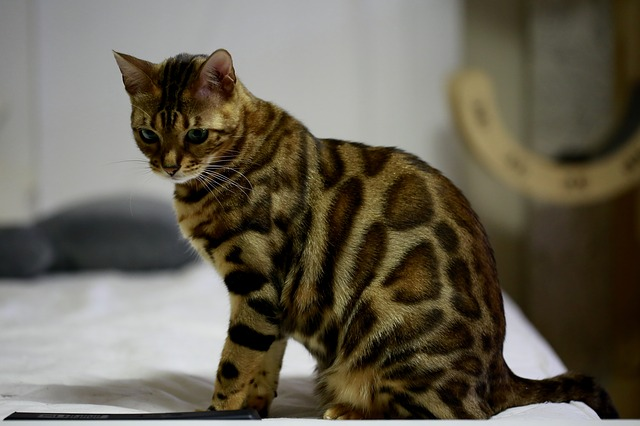
\includegraphics[width=.95\linewidth]{cat.jpg}} %
  \only<2->{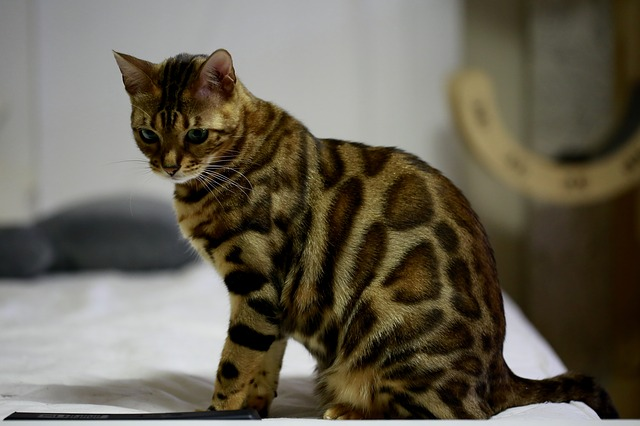
\includegraphics[width=.4\linewidth]{cat.jpg}} \linebreak Felis catus pthr10037 & %
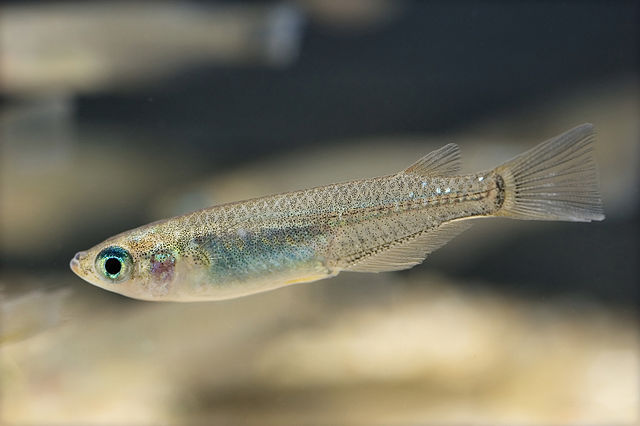
\includegraphics[width=1\linewidth]{Oryzias_latipes.jpg} \linebreak Oryzias latipes \textbf{pthr11521} \\ %
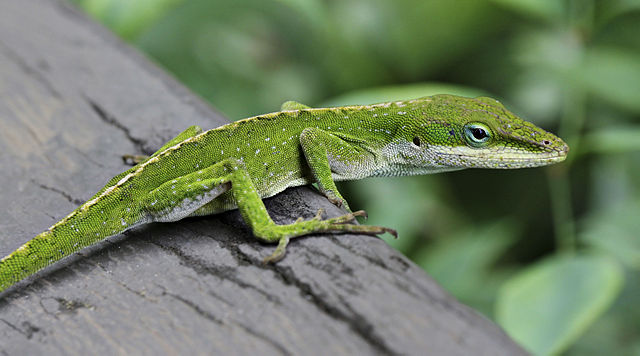
\includegraphics[width=1\linewidth]{Anole_Lizard.jpg} \linebreak Anolis carolinensis \textbf{pthr11521} & %
\only<1>{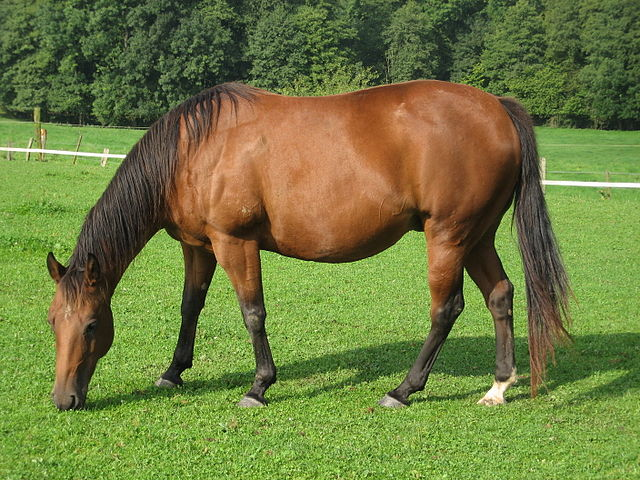
\includegraphics[width=.725\linewidth]{horse.jpg}} %
  \only<2->{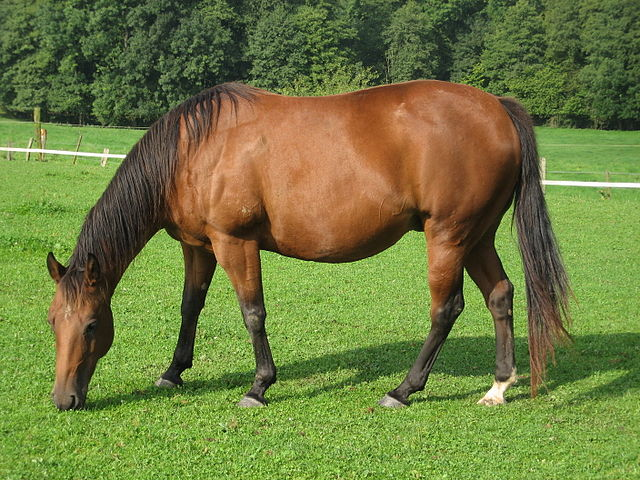
\includegraphics[width=.4\linewidth]{horse.jpg}} \linebreak Equus caballus pthr24356
\end{tabular}
\end{table}

\vfill \hfill \hyperlink{geneontology}{\beamerreturnbutton{go back}}

\end{frame}


% ------------------------------------------------------------------------------
\begin{frame}[label=other-models]
\frametitle{Predicting gene functions}
There various approaches for this, some to highlight
\begin{itemize}%[<+->]
\item Text analysis like in \cite{Pesaranghader2016}
\item Protein-protein interaction networks like in \cite{Oliver2000,Piovesan2015}.
\item Phylogenetic based like SIFTER \cite{Engelhardt2005,Engelhardt2011}.
\begin{itemize}
\item Parameters to estimate: $2^{2P}$, where $P$ is the number of functions.
\end{itemize}
\end{itemize}

\vfill \hfill (a nice literature review in \cite{Jiang2016,Yu2018})
\hyperlink{aphylographicalview}{\beamerreturnbutton{go back}}

\end{frame}


% ------------------------------------------------------------------------------
\begin{frame}[label=aphyloalgorithmicview]
\frametitle{An evolutionary model of gene functions (algorithmic view)}

\scalebox{.7}{

\begin{algorithm}[H]
\SetAlgoLined
\KwData{A phylogenetic tree, $\{\pi, \mu, \psi\}$(Model probabilities)}
\KwResult{An annotated tree}
%\pause
\For{$n \in PostOrder(N)$}{
  $\mbox{\bf\color{usccardinal}Nodes gain/loss function depending on their parent}$\;%\pause
  \Switch{class of $n$}{
    \uCase{root node}{
      Gain function with probability $\pi$\;
    }%\pause
    \uCase{interior node} {%\pause
      \lIf{Parent has the function}{Keep it with prob. $(1-\mu_1)$}%\pause
      \lElse{Gain it with prob. $\mu_0$}%\pause
    }
  }%\pause
  $\mbox{\bf\color{usccardinal}Finally, we allow for mislabeling}$\;%\pause
  \uIf{$n$ is leaf}{%\pause
    \lIf{has the function}{Mislabel with prob. $\psi_1$}%\pause
    \lElse{Mislabel with prob. $\psi_0$}%\pause
  }
}
\end{algorithm}
}

\vfill\hfill \hyperlink{aphylographicalview}{\beamergotobutton{go back}}


\end{frame}

% ------------------------------------------------------------------------------
\begin{frame}[label = duplicationvsspeciation]
\frametitle{Speciation}
\begin{figure}
\centering
\def\svgwidth{.8\linewidth}
\tiny
% Source 
\input{fig/Drosophila_speciation_experiment.pdf_tex}
\caption{\cite{Dodd1989}: After one year of isolation, flies showed a significant level or assortativity in mating (\href{https://commons.wikimedia.org/wiki/File:Drosophila_speciation_experiment.svg}{wikimedia})}
\end{figure}

\vfill\hfill \hyperlink{aphylographicalview}{\beamerreturnbutton{go back}}

\end{frame}

\begin{frame}
\frametitle{Duplication}
\begin{figure}
\centering
\def\svgwidth{.6\linewidth}
\tiny
% Source : https://en.wikipedia.org/wiki/File:Evolution_fate_duplicate_genes_-_vector.svg
\input{fig/Evolution_fate_duplicate_genes_-_vector.pdf_tex}
\caption{A key part of molecular innovation, gene duplication provides opportunity for new functions to emerge (\href{https://en.wikipedia.org/wiki/File:Evolution_fate_duplicate_genes_-_vector.svg}{wikimedia})}
\end{figure}

\vfill\hfill \hyperlink{aphylographicalview}{\beamerreturnbutton{go back}}

\end{frame}

% ------------------------------------------------------------------------------
\begin{frame}[label=aphylopkg]
\frametitle{The \aphylopkg{} R package}

\begin{itemize}
\item Simulation and visualization of annotated phylogenetic trees.
\item Pruning algorithm implemented in C++ using the \texttt{pruner} template library (by-product).
\item Uses metaprogramming (users can specify different formulas).
\item The estimation is done using either Maximum Likelihood, Maximum A Posteriory, or MCMC.
\item The MCMC estimation is done via the \texttt{fmcmc} R package using adaptive MCMC
(also implemented as part of this project):
\begin{itemize}
\item Automatic stop via convergence check.
\item Out-of-the-box parallel chains using parallel computing.
\item User-defined transition kernel (in our case, Adaptive Kernel).
\end{itemize}
\end{itemize}

\vfill\hfill \hyperlink{aphylographicalview}{\beamerreturnbutton{go back}}
\end{frame}



% ------------------------------------------------------------------------------
\begin{frame}[label=mcmle]
\frametitle{ERGMs: The MC-MLE approach}

One of the most popular methods for estimating ERGMs is the MC-MLE approach (citations here)

This consists on the following steps

\begin{enumerate}
\item Start from a sensible guess on what should be the population parameters
(usually done using pseudo-MLE estimation)
\item While the algorithm doesn't converge, do:
  \begin{enumerate}
  \item Simulate a stream of networks with the current state of the parameter,
  $\theta_t$
  \item Using the law of large numbers, approximate the ratio of likelihoods 
  based on the parameter $\theta_t$, this is the objective function
  \item Update the parameter by a Newton-Raphson step
  \item Next iteration
  \end{enumerate}
\end{enumerate}

\vfill\hfill \hyperlink{art}{\beamerreturnbutton{go back}}


\end{frame}

% ------------------------------------------------------------------------------
\begin{frame}[label=ergmitopkg]
\frametitle{The \ergmitopkg{}}

In general

\begin{itemize}
\item Implements estimation of ERGMs using exact statistics for small networks
\item Meta-programming allows specifying likelihood (and gradient) functions for
joint models (a function that writes a function)
\item Includes tools for simulating, and post-estimation checks
\item Getting ready for CRAN!
\end{itemize}

More specific tricks

\begin{itemize}
\item Computes support of Pr using \texttt{ergm::ergm.allstats}
\item It includes a vectorized function doing the same
\item Scales up nice (hundreds of small networks) saving space and computation (when possible)
\item Highly tested (90\% coverage with more than one hundred tests)
\end{itemize}

\vfill\hfill \hyperlink{ergmito}{\beamerreturnbutton{go back}}

\end{frame}

% ------------------------------------------------------------------------------
\begin{frame}[label=ergmitodgp]
\frametitle{Paper 2 Simulation Studies}

We performed a simulation study with the following features:

\begin{itemize}%[<+->]
\item Draw 20,000 samples of groups of small networks
\item Each group had prescribed: (model parameters, number of networks, sizes of the networks)
\item Each group could have from 5 to 300 small networks
\item We estimated the models using MC-MLE and MLE.
\end{itemize}

\vfill\hfill\hyperlink{ergmitoexample}{\beamerreturnbutton{go back}}

\end{frame}



% ------------------------------------------------------------------------------
\begin{frame}[label=ergmito-bias]
\frametitle{Paper 2 Simulation Studies: Empirical Bias}

\begin{figure}
\centering
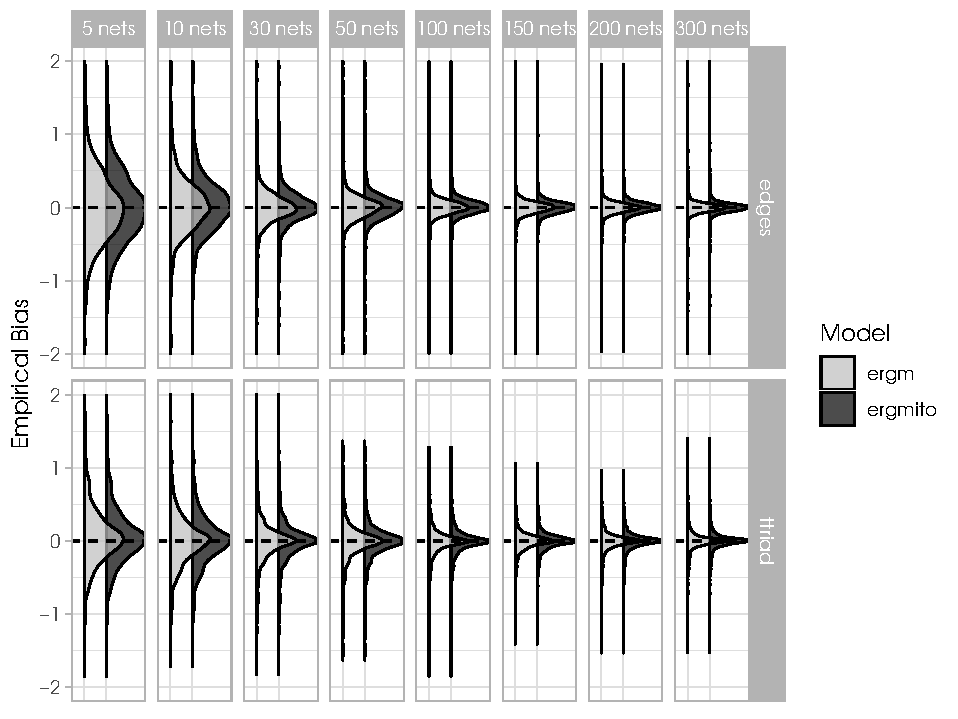
\includegraphics[width=.6\linewidth]{bias-02-various-sizes-4-5-ttriad.pdf}
\end{figure}

\vfill\hfill \hyperlink{ergmitoexperiment}{\beamerreturnbutton{go back}}

\end{frame}

\end{document}

